\section{Enormous untapped potential: integrating mobile devices into the Grid}\label{untapped_enormous_potential}
Now, with a general understanding of what Grid Computing is and how mobile devices evolved over the years, the main topic of this work can be discussed: integrating (using volunteer computing) mobile devices into Grid Computing alongside desktop computers exploiting an enormous quantity of computational resources that lay unused in the pockets of billions of users.

\subsection{Idea: strength in numbers}
As seen in \textit{figure \ref{fig:global_sales_of_pcs_and_smartphones}}, the market has an enormous number of smartphones sold, thus resulting in an abundance of available devices that billions of users use every day (tablets have also to be taken into consideration).
\vspace{10mm}

\begin{figure}[!ht]
    \centering
    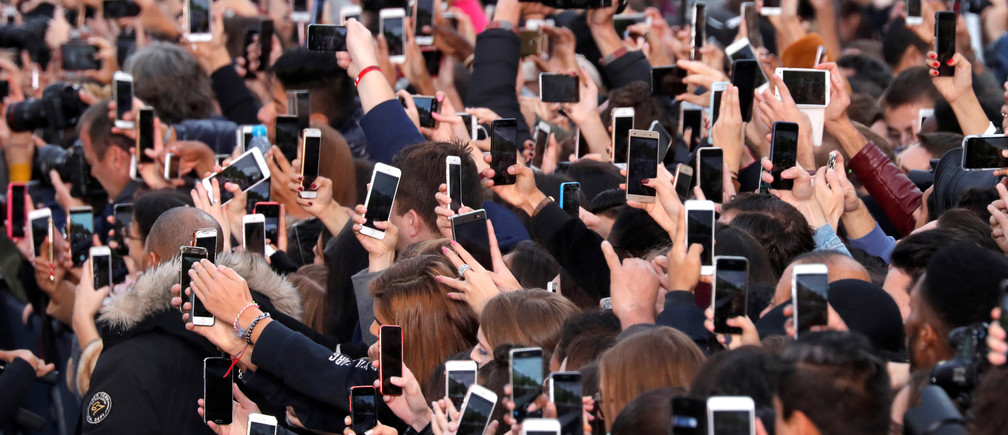
\includegraphics[scale=1.2]{document/chapters/chapter_1/images/people_using_smartphones.jpg}
    \caption{Smartphones are now used daily on a regular basis}
    \label{fig:people_using_smartphones}
\end{figure}

Despite smartphones and tablets are not on the same level (in terms of hardware capabilities) with current computers, it is possible to exploit the availability of a vast number of devices as a leverage to compensate the performances of such mobile devices.
This concept becomes increasingly relevant also considering the tendency of users to progressively use less and less desktop computers in favor of their mobile devices.

\subsection{Previous works and how limitations evolved}
A number of previous works discussed the idea and all of them agreed on the potential of exploiting mobile devices resources; quoting directly from the 2003 article \textit{"Should one incorporate Mobile-ware in Parallel and Distributed Computation?"} by Mustafa Sanver, Sathya Prya Durairaju and Ajay Gupta \cite{should_one_incorporate_mobile_ware}:
\begin{quotation}
    \textit{"At first glance, an individual mobile device may not have sufficient capacity and computational power for the integration. However, if we can harness the aggregated mobile power instead of individual power and consider exponential-rise of mobile units marketed and significantly evolving mobile technology, then one may conclude that it is worth the effort using this vast, pervasive, and untouched computational source for parallel computation."}
\end{quotation}

While recognizing the potential behind this concept, previous works pointed out two important arguments against integrating mobile devices into Grid Computing:
\begin{itemize}
    \item Challenges inherently linked with adding mobile devices to the Grid, that this work will discuss in detail later in \textit{section TODO};
    \item Technical limitations, that will now be discussed in order to show how (mostly) they no longer apply, and thus this idea can be realized.
\end{itemize}

\subsubsection{Mobile devices competitive performances}
The first limitation that was pointed at was the poor performances of mobile devices; while this was certainly true for PDAs, as discussed in \textit{section \ref{technological_progress}}, today's smartphones and tablets do offer resources that are vastly more powerful than what was available in the past.

Wireless connectivity is also much stabler, faster and wildly available, especially considering the possibility of limiting participation in the Grid only while the device is connected to a Wi-Fi network.

The mobility factor of such devices is also not a limiting issue since one could argue that a volunteer that moves its device in space (thus possibly interrupting the connection to the Wi-Fi network) can be assimilated to a desktop volunteer that turns off its computer or is suddenly isolated from the network, reducing the mobility to a challenge inherently tied to Grid Computing.

\subsubsection{Mobile users common behavior}
Users current common behaviors solve two limitations addressed in the past:
\begin{itemize}
    \item \textit{Mobile devices need to be always on to contribute to a Grid}\\
    While this was certainly a problem in the past, in today's normal usage of mobile devices (and with the enhancement of the capabilities of batteries), it is normal to maintain a mobile device on 24/7, alternating cycles of running only on battery power and cycles of recharging said batteries.
    \item \textit{Mobile devices do not possess enough resources to both satisfy its use cases and, simultaneously, contribute to a Grid.}\\
    As explored before, resources in devices are wildly more available today, compared to the past. It could be argued that while capabilities are increased, also resource usage to run computational tasks has increased; while this is true, it must be addressed how those devices are unused for relatively long periods of time (especially in the case of tablets). There is also the fact that the typical mobile user uses its device for relatively light-weighted computational tasks such as browsing the internet and interacting with social media applications, leaving still a great portion of resources unused.
\end{itemize}

\subsubsection{Economically sustainable Internet connections}
In the 2000s, internet access was progressively rising, but Internet service providers still offered their services to consumers with a connection according to a consumption plan; that means that the more data a user consumed, the more expensive the connection fee becomes every month. The problem with the usage of such consumption plan was that it made it expensive for end users to voluntarily offer their devices to participate in a Grid.

Such limitation does not exist anymore since the most common way of accessing the Internet today is by a subscription model. It could be argued that mobile users still get a limited amount of traffic data available each month, therefore they could be reluctant to invest it in the participation in a Grid but, as mentioned before, the participation in the Grid could be limited to only while the mobile device is connected to a Wi-Fi network (that commonly has unlimited access to the Internet).

\subsubsection{Standardized mobile market}
Another important limitation pointed out in the past was poor software interoperability and security of 
mobile devices.

The poor software interoperability at the time was the result of how the mobile market was heterogeneous, especially regarding the operative systems that ran on such devices:
\begin{itemize}
    \item Palm OS;
    \item Microsoft Windows Mobile;
    \item EPOC;
    \item Linux;
    \item Newton;
    \item QNX.
\end{itemize}
Having a multitude of OSes resulted in making the process of integrating the mobile devices into the Grid much more difficult, having to manage multiple implementations compatible with a specific OS. While the OSes panorama was also relatively wide in the first years of the smartphones and tablets era, with time the market slowly converged into having primarily two main operative systems: Android and iOS.

\begin{figure}[!ht]
    \centering
    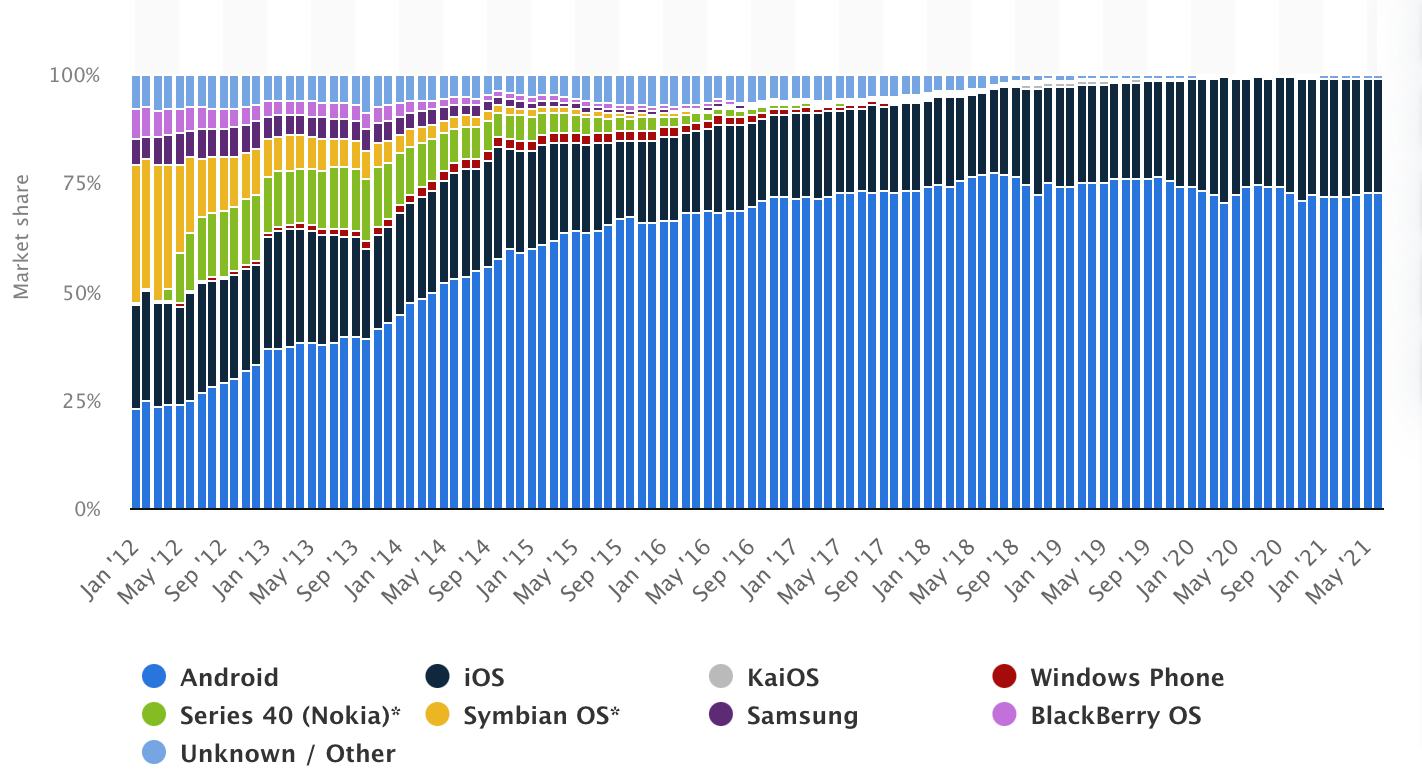
\includegraphics[scale=0.31]{document/chapters/chapter_1/images/os_market_share_2012_to_2021.png}
    \caption{Mobile OSs Market Share from January 2012 to June 2021 \cite{mobile_and_desktop_os_market}}
    \label{fig:os_market_share_2012_to_2021}
\end{figure}

It must also be mentioned that today there are frameworks that allow to have a singular codebase for creating native applications for both Android and iOS, making the maintenance process even simpler.

On the security side having only two real competitors that constantly update their OSes makes the current situation more favorable than the 2000s (while of course additional security measures has to be used).

\subsubsection{Not only mobile: devices transparency principle}
As mentioned in the beginning of \textit{section \ref{untapped_enormous_potential}}, the vision of Grid Computing that this work wants to discuss does not only include mobile devices but continues to also use desktop computers to expand the capabilities that can be achieved.

The coexistence of both mobile devices and computers in the Grid at the same time makes necessary to introduce a devices transparency principle: a node that participates in the Grid is just characterized by the resources it has to offer, independently of the nature of the device. If this principle is respected, while performing tasks inside the Grid, the complexity of having different type of devices disappears, making the process transparent to someone that requests a service from the Grid.
